\chapter{Orbitales atomiques~: formes, énergies et tailles}\label{ch:b2:atomic-orbitals}

Un atome d'hydrogène n'a pas de bord~: son électron peut se trouver à n'importe quelle distance du
noyau, avec une probabilité qui décroît vite mais ne s'annule jamais. Pourtant, les atomes
ont une taille, et un atome de sodium est environ deux fois plus large qu'un atome de
chlore, bien qu'il contienne moins d'électrons. Le volume de première année a nommé les
états d'un électron par trois nombres quantiques~; ici, chacun d'eux devient une
fonction de la position, avec une forme, des nœuds, des signes et une taille, et un jeu simple
de règles en tire les \omterm{def:b2:atomic-orbitals:orbital-energy}{énergies orbitalaires} de n'importe quel atome. Ce sont ces formes et ces signes
que les quatre chapitres suivants combinent en orbitales moléculaires.

\begin{recall}
Le volume de première année~: nombres quantiques $n$, $l$, $m_l$, $m_s$~; les orbitales atomiques comme
états $(n, l, m_l)$~; couches et sous-couches~; effet d'écran et charge nucléaire
effective (qualitativement)~; configurations électroniques~; les niveaux de l'hydrogène,
$-E_R/n^2$ avec $E_R = \qty{13.6}{eV}$. En physique~: la \omterm{def:b2:atomic-orbitals:wavefunction}{fonction d'onde}, dont le
carré du module est une \omterm{def:b2:atomic-orbitals:wavefunction}{densité de probabilité}.
\end{recall}

\section{Les fonctions d'onde de l'atome d'hydrogène}

\begin{definition}[Fonction d'onde]\label{def:b2:atomic-orbitals:wavefunction}
L'état d'un électron est décrit par une \emph{fonction d'onde}\index{fonction d'onde}
$\psi(x, y, z)$~; $|\psi|^2$ est sa \emph{densité de probabilité}\index{densite de probabilite@densité de probabilité}~:
la probabilité de trouver l'électron dans un petit volume $dV$ autour
d'un point vaut $|\psi|^2\,dV$, et $\int|\psi|^2\,dV = 1$ sur tout l'espace (la fonction
est normalisée). Une orbitale atomique est la fonction d'onde d'un électron dans un
atome.
\end{definition}

\begin{definition}[Partie radiale et partie angulaire]\label{def:b2:atomic-orbitals:radial-angular}
En coordonnées sphériques $(r, \theta, \varphi)$ centrées sur le noyau, les orbitales
d'un atome hydrogénoïde se factorisent en $\psi_{nlm}(r, \theta, \varphi) = R_{nl}(r)\,
Y_{lm}(\theta, \varphi)$~: la \emph{partie radiale}\index{partie radiale} $R_{nl}$ dépend
de $n$ et de $l$, la \emph{partie angulaire}\index{partie angulaire} $Y_{lm}$ de $l$ et de
$m_l$ seulement.
\end{definition}

\begin{theorem}[Les orbitales hydrogénoïdes]\label{thm:b2:atomic-orbitals:hydrogen}
Pour un atome à un électron de charge nucléaire $Ze$, avec $\rho = Zr/a_0$ et $a_0 =
\qty{52.9}{pm}$ le rayon de Bohr, les \omterm{def:b2:atomic-orbitals:radial-angular}{parties radiales} pour $n \leq 3$ sont, en unités de
$(Z/a_0)^{3/2}$~:
\[
\begin{array}{ll}
  R_{1s} = 2\,\mathrm e^{-\rho} &
  R_{2s} = \dfrac{1}{2\sqrt2}\,(2 - \rho)\,\mathrm e^{-\rho/2} \\[2ex]
  R_{2p} = \dfrac{1}{2\sqrt6}\,\rho\,\mathrm e^{-\rho/2} &
  R_{3s} = \dfrac{2}{81\sqrt3}\,(27 - 18\rho + 2\rho^2)\,\mathrm e^{-\rho/3} \\[2ex]
  R_{3p} = \dfrac{4}{81\sqrt6}\,(6\rho - \rho^2)\,\mathrm e^{-\rho/3} &
  R_{3d} = \dfrac{4}{81\sqrt{30}}\,\rho^2\,\mathrm e^{-\rho/3}
\end{array}
\]
et les \omterm{def:b2:atomic-orbitals:radial-angular}{parties angulaires} réelles sont $Y_s = 1/\sqrt{4\pi}$~; $Y_{p_x}, Y_{p_y}, Y_{p_z} =
\sqrt{3/(4\pi)}\,(x, y, z)/r$~; $Y_{d_{xy}} = \sqrt{15/(4\pi)}\,xy/r^2$ (et de même
$xz$, $yz$), $Y_{d_{x^2-y^2}} = \sqrt{15/(16\pi)}\,(x^2 - y^2)/r^2$, $Y_{d_{z^2}} =
\sqrt{5/(16\pi)}\,(3z^2 - r^2)/r^2$. Leurs énergies sont $E_n = -Z^2E_R/n^2$.
% ledger: const:a0, const:RyhcEV
\end{theorem}

\admitted

Ces fonctions sont les solutions de l'équation de Schrödinger pour un électron
et un noyau, établies dans le volume de troisième année. Les fonctions $p$ et $d$ réelles sont des
combinaisons des fonctions complexes repérées par $m_l$~; elles pointent selon les axes et
ce sont elles qui servent à construire les liaisons.

\begin{omfigure}
\begin{minipage}[t]{0.27\linewidth}\vspace{0pt}
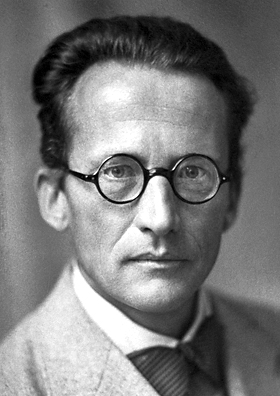
\includegraphics[width=\linewidth]{images/book3/schrodinger.jpg}
\end{minipage}\hfill
\begin{minipage}[t]{0.69\linewidth}\vspace{0pt}
{\small Erwin Schrödinger, qui écrivit en 1926 l'équation d'onde dont les
solutions pour l'atome d'hydrogène sont les orbitales de ce chapitre, et en retrouva
les niveaux d'énergie que Bohr avait postulés. Il partagea le prix Nobel
de physique en 1933. (Photographie~: Fondation Nobel, domaine public,
Wikimedia Commons.)}
\end{minipage}
\end{omfigure}

\section{La partie radiale}

La probabilité de trouver l'électron entre les sphères de rayons $r$ et $r +
dr$ est $|\psi|^2$ intégrée sur la coquille de volume $4\pi r^2\,dr$~; pour toute
orbitale, une fois les angles intégrés, elle vaut $r^2R^2\,dr$.

\begin{definition}[Distribution radiale]\label{def:b2:atomic-orbitals:radial-distribution}
La \emph{fonction de distribution radiale}\index{fonction de distribution radiale} d'une
orbitale est $P(r) = r^2R_{nl}(r)^2$~: $P(r)\,dr$ est la probabilité que
l'électron se trouve entre $r$ et $r + dr$ du noyau. Le \emph{rayon le plus
probable}\index{rayon le plus probable} est la valeur de $r$ correspondant à son plus grand maximum.
\end{definition}

\begin{proposition}[Normalisation de 1s]\label{prop:b2:atomic-orbitals:normalised}
$\int_0^\infty P_{1s}(r)\,dr = 1$.
\end{proposition}

\begin{proof}
Avec $Z = 1$ et $r$ en unités de $a_0$, $P_{1s} = 4r^2\mathrm e^{-2r}$. Par deux intégrations par parties,
$\int_0^\infty r^2\mathrm e^{-2r}\,dr = \frac22\int_0^\infty r\,\mathrm e^{-2r}\,dr =
\frac12\int_0^\infty\mathrm e^{-2r}\,dr = \frac14$, et $4 \times \frac14 = 1$.
\end{proof}

\begin{proposition}[Rayon le plus probable]\label{prop:b2:atomic-orbitals:most-probable}
Pour l'orbitale 1s, le \omterm{def:b2:atomic-orbitals:radial-distribution}{rayon le plus probable} vaut $a_0/Z$. Pour une orbitale telle que $l =
n - 1$ (1s, 2p, 3d, \dots), il vaut $n^2a_0/Z$.
\end{proposition}

\begin{proof}
Pour $l = n - 1$, la \omterm{def:b2:atomic-orbitals:radial-angular}{partie radiale} n'a pas de nœud~: $R \propto \rho^{n-1}\mathrm e^{-\rho/n}$,
donc $P \propto \rho^{2n}\mathrm e^{-2\rho/n}$ et $d\ln P/d\rho = 2n/\rho - 2/n$, nul
pour $\rho = n^2$, c'est-à-dire $r = n^2a_0/Z$. Avec $n = 1$, $r = a_0/Z$.
\end{proof}

\begin{proposition}[Rayon moyen de 1s]\label{prop:b2:atomic-orbitals:mean-radius}
La distance moyenne d'un électron 1s au noyau vaut $\langle r\rangle = 3a_0/(2Z)$,
plus que son \omterm{def:b2:atomic-orbitals:radial-distribution}{rayon le plus probable}.
\end{proposition}

\begin{proof}
Avec $Z = 1$~: $\langle r\rangle = \int_0^\infty r\,P(r)\,dr = 4\int_0^\infty r^3\mathrm e^{-2r}
\,dr = 4 \times 3!/2^4 = 3/2$. La distribution a une longue queue aux grands $r$,
qui entraîne la moyenne au-delà du maximum.
\end{proof}

\begin{definition}[Nœuds]\label{def:b2:atomic-orbitals:node}
Une \emph{surface nodale}\index{surface nodale} d'une orbitale est une surface sur laquelle
la \omterm{def:b2:atomic-orbitals:wavefunction}{fonction d'onde} s'annule en changeant de signe. C'est un \emph{nœud radial}\index{noeud radial@nœud radial}
(une sphère) lorsque la \omterm{def:b2:atomic-orbitals:radial-angular}{partie radiale} s'annule, un \emph{nœud
angulaire}\index{noeud angulaire@nœud angulaire} (un plan ou un cône passant par le noyau) lorsque c'est la \omterm{def:b2:atomic-orbitals:radial-angular}{partie angulaire}
qui s'annule.
\end{definition}

\begin{proposition}[Dénombrer les nœuds]\label{prop:b2:atomic-orbitals:nodes}
Une orbitale $(n, l)$ possède $n - l - 1$ \omterm{def:b2:atomic-orbitals:node}{nœuds radiaux} et $l$ \omterm{def:b2:atomic-orbitals:node}{nœuds angulaires}, $n - 1$ en
tout.
\end{proposition}

\begin{proof}
Sur les fonctions du \cref{thm:b2:atomic-orbitals:hydrogen}~: $R_{2s}$ s'annule en
$\rho = 2$, $R_{3s}$ aux deux racines de $2\rho^2 - 18\rho + 27$ ($\rho = 1.90$ et $7.10$),
$R_{3p}$ en $\rho = 6$~; $R_{1s}$, $R_{2p}$, $R_{3d}$ ne s'annulent pas. La \omterm{def:b2:atomic-orbitals:radial-angular}{partie angulaire}
d'une orbitale p s'annule sur un plan ($z = 0$ pour $p_z$), celle d'une orbitale d sur deux
plans ou, pour $d_{z^2}$, sur un cône. Le cas général est admis.
\end{proof}

\begin{omfigure}
\begin{tikzpicture}
\begin{axis}[width=0.55\linewidth, height=6cm, xmin=0, xmax=24, ymin=0, ymax=0.58,
  axis x line=bottom, axis y line=left, xlabel={$r/a_0$}, ylabel={$P(r)$},
  tick label style={font=\small}, label style={font=\small}, title={\small distributions radiales, $Z = 1$}]
\addplot[omThm, thick] table[x=r, y=s1] {figdata/out/bachelor-2-atomic-orbitals-a.dat};
\addplot[omDef, thick] table[x=r, y=s2] {figdata/out/bachelor-2-atomic-orbitals-a.dat};
\addplot[omDef, thick, dashed] table[x=r, y=p2] {figdata/out/bachelor-2-atomic-orbitals-a.dat};
\addplot[omProp, thick] table[x=r, y=s3] {figdata/out/bachelor-2-atomic-orbitals-a.dat};
\addplot[omProp, thick, dashed] table[x=r, y=p3] {figdata/out/bachelor-2-atomic-orbitals-a.dat};
\addplot[omProp, thick, dotted] table[x=r, y=d3] {figdata/out/bachelor-2-atomic-orbitals-a.dat};
\node[font=\scriptsize, omThm, anchor=west] at (axis cs:1.4,0.53) {1s};
\node[font=\scriptsize, omDef, anchor=south] at (axis cs:4.0,0.215) {2p};
\node[font=\scriptsize, omDef, anchor=south west] at (axis cs:6.4,0.17) {2s};
\node[font=\scriptsize, omProp, anchor=south] at (axis cs:10.5,0.12) {3d};
\node[font=\scriptsize, omProp, anchor=west] at (axis cs:17,0.085) {3s, 3p};
\end{axis}
\end{tikzpicture}\hfill
\begin{tikzpicture}
\begin{axis}[width=0.42\linewidth, height=6cm, xmin=0, xmax=20, ymin=-0.12, ymax=0.75,
  axis x line=middle, axis y line=left, xlabel={$r/a_0$}, ylabel={$R$},
  tick label style={font=\small}, label style={font=\small}, title={\small parties radiales}]
\addplot[omDef, thick] table[x=r, y=R2s] {figdata/out/bachelor-2-atomic-orbitals-b.dat};
\addplot[omProp, thick] table[x=r, y=R3s] {figdata/out/bachelor-2-atomic-orbitals-b.dat};
\node[font=\scriptsize, omDef, anchor=west] at (axis cs:0.4,0.62) {$R_{2s}$};
\node[font=\scriptsize, omProp, anchor=west] at (axis cs:0.6,0.30) {$R_{3s}$};
\node[font=\scriptsize, anchor=south west] at (axis cs:3,0.15) {nœud};
\draw[thin, ->] (axis cs:3,0.15) -- (axis cs:2.05,0.01);
\end{axis}
\end{tikzpicture}

{\small À gauche~: distributions radiales $P(r) = r^2R^2$ des orbitales de l'hydrogène jusqu'à
$n = 3$~; plus $n$ est grand, plus l'électron est loin, et les orbitales s ont de
petits maximums internes (pénétration). À droite~: $R_{2s}$ et $R_{3s}$ changent de signe à leurs
\omterm{def:b2:atomic-orbitals:node}{nœuds radiaux} ($r = 2a_0$~; $1.90a_0$ et $7.10a_0$).}
\end{omfigure}

\begin{omfigure}
\begin{tikzpicture}
\begin{axis}[scale only axis, width=0.32\linewidth, height=0.32\linewidth,
  xmin=-6, xmax=6, ymin=-6, ymax=6, axis lines=none, title={\small 1s}]
\addplot[only marks, mark=*, mark size=0.25pt, omDef] table[x=x, y=y] {figdata/out/bachelor-2-atomic-orbitals-c-1s.dat};
\end{axis}
\end{tikzpicture}\hspace{0.12\linewidth}%
\begin{tikzpicture}
\begin{axis}[scale only axis, width=0.32\linewidth, height=0.32\linewidth,
  xmin=-14, xmax=14, ymin=-14, ymax=14, axis lines=none, title={\small 2s}]
\addplot[only marks, mark=*, mark size=0.25pt, omDef] table[x=x, y=y] {figdata/out/bachelor-2-atomic-orbitals-c-2s.dat};
\draw[densely dashed, omThm] (axis cs:0,0) circle[radius=2];
\end{axis}
\end{tikzpicture}

{\small Représentations en densité de points des orbitales 1s et 2s de l'hydrogène dans un plan
passant par le noyau~: la densité de points suit $|\psi|^2$ (échantillonnage
déterministe). Le nuage 2s présente un anneau vide, le \omterm{def:b2:atomic-orbitals:node}{nœud radial} à $2a_0$ (en tirets)~;
les cadres ont une largeur de 12 et 28 $a_0$.}
\end{omfigure}

\section{La partie angulaire}

La \omterm{def:b2:atomic-orbitals:radial-angular}{partie angulaire} fixe la forme. Une orbitale s est sphérique~; une orbitale p possède deux
lobes de signes opposés le long de son axe, séparés par un plan nodal~; une orbitale d possède
quatre lobes de signes alternés (ou, pour $d_{z^2}$, deux lobes et un anneau). Le signe
d'un lobe n'a pas de sens physique en lui-même --- $\psi$ et $-\psi$ décrivent le même
état --- mais les signes relatifs de deux orbitales décident, au chapitre suivant,
si elles se combinent en une liaison.

\begin{omfigure}
\begin{tikzpicture}[font=\small]
  \pic at (0,0) {oms={1}};
  \node[below] at (0,-0.75) {s};
  \pic at (2.0,0) {omp={1}{0}};
  \draw[->, black!55, thin] (1.0,0) -- (3.0,0) node[right, font=\tiny] {$x$};
  \node[below] at (2.0,-0.75) {$\mathrm p_x$};
  \pic at (4.2,0) {omp={1}{90}};
  \draw[->, black!55, thin] (4.2,-0.95) -- (4.2,0.95) node[above, font=\tiny] {$z$};
  \node[below] at (4.75,-0.75) {$\mathrm p_z$};
  \pic at (6.6,0) {omdxy}; \node[below] at (6.6,-1.0) {$\mathrm d_{xy}$};
  \pic at (9.0,0) {omdx2y2}; \node[below] at (9.0,-1.0) {$\mathrm d_{x^2-y^2}$};
  \pic at (11.4,0) {omdz2}; \node[below] at (11.4,-1.0) {$\mathrm d_{z^2}$};
\end{tikzpicture}

{\small Orbitales atomiques réelles, schéma~: les lobes figurent les régions où $|\psi|$
est grand, colorées selon le signe de $\psi$ (bleu positif, orange négatif). Les
orbitales $\mathrm d_{xz}$ et $\mathrm d_{yz}$ ont la forme de $\mathrm d_{xy}$ dans
les plans que désignent leurs noms.}
\end{omfigure}

\begin{method}[Représenter une orbitale à partir de ses nombres quantiques]\label{met:b2:atomic-orbitals:draw-orbital}
\begin{enumerate}
  \item D'après $l$, la forme~: s (sphère), p (deux lobes), d (quatre lobes, ou deux
        lobes et un anneau pour $d_{z^2}$)~; d'après l'indice, l'orientation.
  \item Compter les $l$ \omterm{def:b2:atomic-orbitals:node}{nœuds angulaires} (plans passant par le noyau) et donner
        aux lobes adjacents des signes opposés.
  \item Compter les $n - l - 1$ \omterm{def:b2:atomic-orbitals:node}{nœuds radiaux}~: des coquilles internes de signe opposé à l'intérieur
        des lobes principaux (en général omises dans les schémas).
  \item Mettre à l'échelle avec $n^2a_0/Z$~: plus $n$ est grand, plus l'orbitale est grande~; plus $Z$ est grand, plus elle est petite.
\end{enumerate}
\end{method}

\section{Les atomes polyélectroniques}

Dans un atome à plusieurs électrons, chaque électron perçoit le noyau écranté par
les autres. Les orbitales gardent la forme de celles de l'hydrogène, avec une charge
effective $Z^*$ à la place de $Z$, et l'énergie d'une sous-couche dépend maintenant de $l$
autant que de $n$~: un électron s, dont la distribution radiale présente des maximums internes proches
du noyau, est moins écranté qu'un électron p de la même couche, et un p moins
qu'un d.

\begin{definition}[Règles de Slater]\label{def:b2:atomic-orbitals:slater}
Les \emph{règles de Slater}\index{regles de Slater@règles de Slater} estiment la charge nucléaire effective
$Z^* = Z - \sigma$ perçue par un électron. Les électrons sont regroupés en
(1s) (2s, 2p) (3s, 3p) (3d) (4s, 4p) (4d) (4f) (5s, 5p) \dots~; la constante
d'écran $\sigma$ d'un électron est la somme des contributions des autres
électrons~: 0.35 pour chaque autre électron du même groupe (0.30 au sein de 1s)~;
pour un électron s ou p, 0.85 pour chaque électron de la couche $n - 1$ et 1.00 pour
chaque électron des couches inférieures~; pour un électron d ou f, 1.00 pour chaque électron
des groupes situés au-dessous du sien. Les groupes supérieurs ne contribuent pas.
\end{definition}

\begin{omfigure}
\small
\renewcommand{\arraystretch}{1.2}
\begin{tabular}{l|ccccc}
électron étudié & même groupe & couche $n - 1$ & couches inférieures & groupes supérieurs \\ \hline
1s & 0.30 & --- & --- & 0 \\
$n$s, $n$p & 0.35 & 0.85 & 1.00 & 0 \\
$n$d, $n$f & 0.35 & 1.00 & 1.00 & 0 \\
\end{tabular}

\smallskip
{\small Constantes d'écran de Slater, par électron écrantant. Les nombres quantiques
principaux effectifs sont $n^* = 1, 2, 3, 3.7, 4.0, 4.2$ pour $n = 1$ à 6.}
\end{omfigure}

\begin{method}[Calculer une charge effective]\label{met:b2:atomic-orbitals:slater}
\begin{enumerate}
  \item Écrire la configuration selon les groupes de Slater, par ordre de $n$, s et p
        ensemble, d et f à part.
  \item Choisir l'électron~; ajouter 0.35 pour chaque autre électron de son groupe.
  \item Ajouter 0.85 (électron s ou p) ou 1.00 (d ou f) par électron de la couche
        immédiatement inférieure, et 1.00 par électron plus profond.
  \item $Z^* = Z - \sigma$.
\end{enumerate}
\end{method}

\begin{definition}[Énergie et rayon orbitalaires]\label{def:b2:atomic-orbitals:orbital-energy}
Dans le modèle de Slater, l'\emph{énergie orbitalaire}\index{energie orbitalaire@énergie orbitalaire} d'un électron
de charge effective $Z^*$ et de nombre quantique principal effectif $n^*$ vaut
$\varepsilon = -E_RZ^{*2}/n^{*2}$, et son \emph{rayon orbitalaire}\index{rayon orbitalaire}
vaut $n^{*2}a_0/Z^*$, le \omterm{def:b2:atomic-orbitals:radial-distribution}{rayon le plus probable} d'une orbitale hydrogénoïde de charge
$Z^*$.
\end{definition}

\begin{proposition}[Énergies de Slater]\label{prop:b2:atomic-orbitals:slater-energy}
L'énergie d'un groupe de $k$ électrons de charge effective $Z^*$ vaut approximativement
$k\varepsilon = -kE_RZ^{*2}/n^{*2}$, et l'énergie électronique totale de l'atome
est la somme sur ses groupes.
\end{proposition}

\admitted

\begin{example}[Le fer~: 4s ou 3d d'abord~?]\label{ex:b2:atomic-orbitals:iron}
Le fer est $[\ce{Ar}]\,3\mathrm d^6\,4\mathrm s^2$. Un électron 4s~: $\sigma = 0.35 + 14
\times 0.85 + 10 \times 1.00 = 22.25$, $Z^* = 3.75$, $\varepsilon = -13.6 \times
3.75^2/3.7^2 = \qty{-14.0}{eV}$. Un électron 3d~: $\sigma = 5 \times 0.35 + 18 \times 1.00 =
19.75$, $Z^* = 6.25$, $\varepsilon = -13.6 \times 6.25^2/9 = \qty{-59}{eV}$. Les électrons 3d
sont bien plus fortement liés~: bien que la sous-couche 4s se remplisse la première dans
l'ordre de remplissage, c'est un électron 4s qui part quand on ionise le fer, et l'ion
fer(II) est $[\ce{Ar}]\,3\mathrm d^6$.
\end{example}

\section{Utiliser les énergies et les rayons orbitalaires}

\begin{proposition}[Énergie d'ionisation et énergies de Slater]\label{prop:b2:atomic-orbitals:ionisation}
Dans le modèle de Slater, l'énergie de première ionisation d'un atome est la différence
entre les énergies totales de l'ion et de l'atome, calculées groupe par groupe
avec les charges effectives de chacun.
\end{proposition}

\begin{proof}
L'énergie d'ionisation vaut $E(\text{ion}) - E(\text{atome})$~; d'après la
\cref{prop:b2:atomic-orbitals:slater-energy}, ce sont deux sommes d'énergies de groupes, et
seul le groupe qui perd l'électron change (les groupes internes ne sont pas écrantés par
les électrons externes).
\end{proof}

\begin{example}[Le carbone]\label{ex:b2:atomic-orbitals:carbon}
Carbone, (2s, 2p)$^4$~: $Z^* = 6 - 2 \times 0.85 - 3 \times 0.35 = 3.25$~; l'énergie du groupe vaut
$4 \times (-13.6 \times 3.25^2/4) = \qty{-143.6}{eV}$. L'ion \ce{C+}, (2s, 2p)$^3$~: $Z^* =
3.60$, $3 \times (-13.6 \times 3.60^2/4) = \qty{-132.2}{eV}$. L'énergie d'ionisation vaut
\qty{11.5}{eV}, contre \qty{11.26}{eV} mesurés.
% ledger: ie:C, const:RyhcEV
\end{example}

\begin{omfigure}
\begin{tikzpicture}
\begin{axis}[width=0.47\linewidth, height=5.4cm, xmin=0.5, xmax=8.5, ymin=0, ymax=6.5,
  axis x line=bottom, axis y line=left, xtick={1,2,3,4,5,6,7,8},
  xticklabels={Li,Be,B,C,N,O,F,Ne}, tick label style={font=\small},
  label style={font=\small}, title={\small période 2}]
\addplot[omThm, thick, mark=*, mark size=1.3pt] table[x=k, y=zs] {figdata/out/bachelor-2-atomic-orbitals-d-period.dat};
\addplot[omDef, thick, mark=square*, mark size=1.3pt] table[x=k, y=r] {figdata/out/bachelor-2-atomic-orbitals-d-period.dat};
\node[font=\scriptsize, omThm, anchor=south east] at (axis cs:7.8,5.3) {$Z^*$};
\node[font=\scriptsize, omDef, anchor=south west] at (axis cs:1.2,3.1) {rayon ($a_0$)};
\end{axis}
\end{tikzpicture}\hfill
\begin{tikzpicture}
\begin{axis}[width=0.47\linewidth, height=5.4cm, xmin=1.5, xmax=6.5, ymin=0, ymax=9,
  axis x line=bottom, axis y line=left, xtick={2,3,4,5,6},
  xticklabels={Li,Na,K,Rb,Cs}, tick label style={font=\small},
  label style={font=\small}, title={\small groupe 1}]
\addplot[omThm, thick, mark=*, mark size=1.3pt] table[x=n, y=zs] {figdata/out/bachelor-2-atomic-orbitals-d-group.dat};
\addplot[omDef, thick, mark=square*, mark size=1.3pt] table[x=n, y=r] {figdata/out/bachelor-2-atomic-orbitals-d-group.dat};
\node[font=\scriptsize, omThm, anchor=north] at (axis cs:4,2.0) {$Z^*$};
\node[font=\scriptsize, omDef, anchor=west] at (axis cs:2.1,5.4) {rayon ($a_0$)};
\end{axis}
\end{tikzpicture}

{\small Charge effective de Slater de l'électron de valence et \omterm{def:b2:atomic-orbitals:orbital-energy}{rayon orbitalaire}
$n^{*2}a_0/Z^*$. Le long de la période 2, $Z^*$ augmente de 0.65 par élément et les atomes
se contractent~; en descendant le groupe 1, $Z^*$ reste à 1.30 puis 2.20 tandis que $n^*$ augmente, et les atomes
grossissent.}
\end{omfigure}

Le modèle reproduit les tendances du volume de première année. Le long d'une période, chaque
proton ajouté n'est écranté que pour 0.35 par l'électron ajouté avec lui~: $Z^*$ augmente,
l'orbitale externe se contracte et lie plus fortement. En descendant un groupe, $Z^*$ varie à peine
tandis que la couche externe s'éloigne~: les atomes grossissent et leurs énergies d'ionisation
diminuent. Le sodium, avec $Z^* = 2.20$ pour son électron 3s, a un \omterm{def:b2:atomic-orbitals:orbital-energy}{rayon orbitalaire} de
$9/2.2 = 4.1a_0$~; le chlore, avec $Z^* = 6.10$ pour un électron 3p, $9/6.1 = 1.5a_0$.

\section{Exercices}

\begin{exercise}[$\star$]\label{exo:b2:atomic-orbitals:1}
Donner les nombres quantiques $n$ et $l$, le nombre de \omterm{def:b2:atomic-orbitals:node}{nœuds radiaux} et de \omterm{def:b2:atomic-orbitals:node}{nœuds
angulaires} d'une orbitale 3p et d'une orbitale 4d.
\end{exercise}

\begin{exercise}[$\star$]\label{exo:b2:atomic-orbitals:2}
Montrer à partir de $R_{2p}$ que le \omterm{def:b2:atomic-orbitals:radial-distribution}{rayon le plus probable} d'un électron 2p de l'hydrogène vaut
$4a_0$, et le donner en picomètres.
\end{exercise}

\begin{exercise}[$\star$]\label{exo:b2:atomic-orbitals:3}
Calculer la probabilité de trouver l'électron 1s de l'hydrogène plus près du
noyau que $a_0$.
\end{exercise}

\begin{exercise}[$\star$]\label{exo:b2:atomic-orbitals:4}
Représenter l'orbitale $3\mathrm d_{xy}$~: lobes, signes, plans nodaux. Combien de \omterm{def:b2:atomic-orbitals:node}{nœuds radiaux}
possède-t-elle~?
\end{exercise}

\begin{exercise}[$\star\star$]\label{exo:b2:atomic-orbitals:5}
Calculer la charge effective de Slater d'un électron 2p de l'oxygène et le \omterm{def:b2:atomic-orbitals:orbital-energy}{rayon
orbitalaire} qu'elle donne.
\end{exercise}

\begin{exercise}[$\star\star$]\label{exo:b2:atomic-orbitals:6}
À l'aide de l'exemple du fer, expliquer pourquoi la configuration de \ce{Fe^3+} est
$[\ce{Ar}]\,3\mathrm d^5$ et non $[\ce{Ar}]\,3\mathrm d^3 4\mathrm s^2$.
\end{exercise}

\begin{exercise}[$\star\star$]\label{exo:b2:atomic-orbitals:7}
Estimer par les \omterm{def:b2:atomic-orbitals:slater}{règles de Slater} les énergies de première ionisation du lithium et du sodium,
et comparer aux valeurs mesurées, 5.39 et \qty{5.14}{eV}. Commenter.
\end{exercise}

\begin{exercise}[$\star\star$]\label{exo:b2:atomic-orbitals:8}
Calculer $Z^*$ et le \omterm{def:b2:atomic-orbitals:orbital-energy}{rayon orbitalaire} de l'électron externe du sodium et du
chlore, et expliquer pourquoi l'atome de sodium est le plus gros.
\end{exercise}

\begin{exercise}[$\star\star$]\label{exo:b2:atomic-orbitals:9}
Montrer que les orbitales 1s et 2s de l'hydrogène sont orthogonales,
$\int\psi_{1s}\psi_{2s}\,dV = 0$.
\end{exercise}

\begin{exercise}[$\star\star\star$]\label{exo:b2:atomic-orbitals:10}
Écrire $R_{2p} = N\rho\,\mathrm e^{-\rho/2}$ et déterminer la constante $N$ qui la normalise
($Z = 1$, $r$ en unités de $a_0$).
\end{exercise}

\begin{exercise}[$\star\star\star$]\label{exo:b2:atomic-orbitals:11}
Comparer le rayon moyen et le \omterm{def:b2:atomic-orbitals:radial-distribution}{rayon le plus probable} d'un électron 1s, et
expliquer à partir de l'allure de $P(r)$ pourquoi ils diffèrent.
\end{exercise}

\begin{exercise}[$\star\star\star$]\label{exo:b2:atomic-orbitals:12}
Trouver la \omterm{def:b2:atomic-orbitals:node}{surface nodale} de l'orbitale $\mathrm p_z$ et montrer que $\psi_{2p_z}$
change de signe à sa traversée. Que vaut la \omterm{def:b2:atomic-orbitals:wavefunction}{densité de probabilité} sur cette surface~?
\end{exercise}

\clearpage
\enlargethispage{3\baselineskip}
\section{Problème~: où est l'électron~?}

\begin{problem}[{Problème du week-end --- l'orbitale 1s de l'hydrogène et ses rayons,
la probabilité de trouver l'électron au-delà d'une distance donnée, les nœuds et
les maximums de 2s et de 2p, et l'estimation de Slater des énergies d'ionisation du carbone,
de l'azote et de l'oxygène}]
\label{pb:b2:atomic-orbitals:1}
Données~: $a_0 = \qty{52.9}{pm}$~; $E_R = \qty{13.6}{eV}$~; énergies de première ionisation
mesurées (\unit{eV})~: C 11.26, N 14.53, O 13.62. $\psi_{1s} = \pi^{-1/2}a_0^{-3/2}\,
\mathrm e^{-r/a_0}$.
% ledger: const:a0, const:RyhcEV, ie:C, ie:N, ie:O

\medskip
\noindent\textbf{Partie I --- L'orbitale 1s.}
\begin{enumerate}
  \item Vérifier que $\psi_{1s}$ est normalisée, en utilisant $dV = 4\pi r^2\,dr$.
  \item Écrire la \omterm{def:b2:atomic-orbitals:radial-distribution}{fonction de distribution radiale} $P(r)$.
  \item Déterminer le \omterm{def:b2:atomic-orbitals:radial-distribution}{rayon le plus probable}.
  \item Calculer le rayon moyen.
  \item Pourquoi la moyenne est-elle supérieure au \omterm{def:b2:atomic-orbitals:radial-distribution}{rayon le plus probable}~?
  \item La \omterm{def:b2:atomic-orbitals:wavefunction}{densité de probabilité} est maximale au noyau, et pourtant $P(0) = 0$.
        Expliquer.
  \item Donner le \omterm{def:b2:atomic-orbitals:radial-distribution}{rayon le plus probable} en picomètres.
\end{enumerate}

\medskip
\noindent\textbf{Partie II --- Au-delà d'un rayon.}
\begin{enumerate}[resume]
  \item Montrer que la probabilité de trouver l'électron au-delà de $r_0 =
        xa_0$ vaut $\mathrm e^{-2x}(1 + 2x + 2x^2)$.
  \item La calculer pour $r_0 = a_0$.
  \item La calculer pour $r_0 = 2a_0$.
  \item Trouver par essais successifs le rayon de la sphère qui contient l'électron avec une
        probabilité de 0.90.
  \item En quel sens un atome n'a-t-il pas de bord, et en quel sens a-t-il une taille~?
\end{enumerate}

\medskip
\noindent\textbf{Partie III --- 2s et 2p.}
\begin{enumerate}[resume]
  \item Donner les nœuds de 2s et de 2p (nombre, nature, position).
  \item Où $R_{2s}$ change-t-elle de signe~?
  \item Déterminer le \omterm{def:b2:atomic-orbitals:radial-distribution}{rayon le plus probable} de 2p.
  \item Trouver les deux maximums de $P_{2s} \propto r^2(2 - r)^2\mathrm e^{-r}$ ($r$ en unités de
        $a_0$).
  \item De 2s et de 2p, laquelle présente une densité électronique plus proche du noyau~? Qu'est-ce
        que cela implique dans un atome polyélectronique~?
  \item Comment ces rayons changent-ils pour l'ion hydrogénoïde \ce{C^5+}~?
\end{enumerate}

\medskip
\noindent\textbf{Partie IV --- Carbone, azote, oxygène.}
\begin{enumerate}[resume]
  \item Calculer le $Z^*$ de Slater d'un électron 2p dans C, N et O.
  \item Calculer les \omterm{def:b2:atomic-orbitals:orbital-energy}{énergies orbitalaires} correspondantes.
  \item Estimer l'énergie de première ionisation du carbone comme différence d'énergies
        de groupes.
  \item Même question pour l'azote.
  \item Même question pour l'oxygène, et comparer les trois aux valeurs mesurées.
  \item Quelle particularité des valeurs mesurées le modèle manque-t-il, et pourquoi~?
  \item Donner la probabilité de trouver l'électron 1s de l'hydrogène au-delà
        de $2a_0$.
\end{enumerate}
\end{problem}
